\chapter{P2P MMVE state management and persistency}
\label{p2p_MMVE_state_persistency}
%%%%%%%%%%%%%%%%%%%%%%%%%%%%%%%%%%%%%%%%%%%%%%%%%%%%%%%%%%%%%%%%%%%%%%%

\section{Introduction}

While the previous chapter broadly introduced all the concepts of state consistency, this chapter will focus solely on state management and state persistency in P2P MMVEs. The implementation of state management and persistency in P2P MMVEs allows for the storage of game data. The fact that game data must now be distributed amongst various peers in the network creates challenges not usually present in classic C/S MMVEs.

This chapter classifies the techniques used in documented P2P MMVE architectures and discusses the advantages and disadvantages of the different types of storage. The chapter also shows that no current storage type is well suited to P2P MMVEs. As the field of P2P MMVEs is a growing one, it is believed that a comprehensive survey of storage techniques is required to act as a basis for further research into the field. To the best of our knowledge, such a classification, where a focus is placed specifically on state management and persistency in P2P MMVEs, has not been undertaken in the literature.

This chapter identifies storage techniques used in P2P MMVEs. To achieve state management and persistency in P2P MMVEs, a type of distributed storage is required. Two classic distributed storage architectures are the Network File System (NFS) \cite{NFS4_protocol} and Coda  \cite{Kistler_Coda_disconnected}. There are, however, some major differences between the requirements of a P2P storage model and the classic distributed file storage model.

Firstly, NFS and Coda still require servers. One of the main advantages of P2P MMVEs is that servers are, for the most part, not required. The other requirement is low latency file storage and retrieval, discussed in Section \ref{char_responsiveness}, which NFS and Coda also do not address. Conflicts are also an issue with the Coda system, which allows multiple nodes to modify the same object. Despite the many differences, the divergent applications share some of the same requirements, namely: scalability, reliability, security and responsiveness.

The requirement of disconnected operation is generally not applicable to most interactive online games, where a player has to stay connected to the world, to be able to interact with it. One area where disconnected operation is of interest to game state management and persistency is in the area of mobile gaming. A major challenge for mobile games is the large variances in network latency. Such networks require games that are resistent to network jitter.

One approach has been proposed in \cite{Chandler_disconnected_games}, where every game client serialises its game state and distributes this game state to all other clients. Each client then creates some target game state from all received game states as well as its own state. The game client then attempts to manipulate all NPCs in the game in order to achieve the target game state. The target game state is constantly updated and thus remains a moving target. This is a new type of consistency model with many research opportunities.

\section{State management and state persistency}
A discussion of state storage requires an understanding of the difference between state management and state persistency. These terms are regularly confused in the literature and sometimes one is used where the other is more appropriate. Other times, authors describe both mechanisms as if it is all part of the same model.

In this work, state persistency is defined to mean long term data storage. Meaning that if a server or client goes off-line, the state persistency mechanism will ensure the safe storage of the state for when the server or client starts up again. State persistency is, therefore, storage in secondary persistent memory. All servers require state persistency to back-up the VE state in case of some outage or in case a server restart is required. This storage type does not have to be fast, but it has to be reliable. State persistency in P2P MMVEs is therefore taken to mean the same. It does not have to be fast, but when a client logs out of the VE and logs back in again, the stored state should remain.

State management on the other hand is defined to mean the storage of the VE state in primary memory. This is the state with which the server and clients will interact. It is the state that will be displayed to the agent on the client and it is the state that will require fast reads and writes as consequences of received events or updates. Every time an object update is generated, it will be applied to the objects by state management. Every time the game logic requires the information of other objects to determine which update to generate on account of a received event, it will make use of state management.

Although these are two different types of storage, with different storage requirements, there are also aspects of state management and persistency that are the same. The similarities and differences will be reviewed in Section \ref{key_challenges_cm}. The similarities between state management and state persistency are explained in this chapter by using the generic term ``storage''. There are many ``storage types'' that will be introduced in this chapter. These storage types can either be state management or state persistency. The relevance of difference storage types to state management and consistency will, however, be discussed.

\section{Client/Multi-Server state management and persistency models}
\label{cms_models}

This section introduces the classic state management and persistency architectures used in server cluster or client/muli-server based systems \cite{Hu_voronoi_IM}.

\subsection{Sharding}

A storage model where the VE state is duplicated over multiple servers, with players connecting to one of these servers is termed ``sharding''. Clients are not able to interact or communicate with players on other shards, which reduces game immersion. This method does, however, allow for a more scalable system as maximum load is fixed.

Players are not able to enter a shard if that shard has reached its capacity. In the past, this has caused unhappiness amongst players, since popular
shards could be difficult to log in to. Players are also reluctant to move to a new shard, because a lot of time is invested in their characters in
their ``home'' shard. Sharding doesn't allocate resources efficiently, as one shard may be overpopulated while another is underpopulated. For all
practical purposes, this approach is still merely a C/S approach, with players forced into a specific C/S environment.

The benefit of sharding is its ease of implementation and the reduction of content designer load. Because no inter-server communication is required
and no server migration is supported, this method greatly simplifies the server design process. Another benefit of sharding is that it allows for a
relatively small game world to support many players because of the duplication of the worlds. This reduces the load on level designers and content
designers, who now have to populate a much smaller world with content.

\subsection{Replication-based}
%Redundant
The replication-based model is similar to sharding, with the difference that all servers share the same duplicated game state. Each server contains
the global game state and clients connect to any one of these servers (mirror-servers \cite{mirrored_server}) or through a load distribution
algorithm to a server (proxy-servers \cite{proxy_server_dist}). Each server handles all actions from clients and updates its own database. The
servers in turn send updates to each other over a high quality link, such as fibre, to maintain database consistency at high speeds.

The problem with this system is that the world is never truly consistent and that there are no optimally chosen inconsistency obfuscation boundaries.
In other words, two players standing next to each other in the virtual world, might be on different servers and, therefore, experience two slightly
different worlds.

\subsection{Object-based}
%Object based
The object-based storage model equally distributes all in-game objects amongst the servers \cite{object_based_consistency1}, \cite{object_based_consistency2}, \cite{object_based_consistency3}. For an MMVE, most of these objects are expected to be player objects. The advantage of this method is that the system load is fixed for a certain player population and that the load is equally distributed amongst all servers. This allows for more accurate prediction and provisioning of resources, but still does not handle transient loads
well.

Another issue is inter-server communications for this architecture. The inter-server communications are random and also more than the inter-server
communications for a region based system. The reason for this is that the number of player interactions increase with a decrease in the distance
between the players. Players playing together move together, chat and interact with NPCs together. For a region based model, all player-neighbour
interactions remain local to the server.

\subsection{Zone/Region-based}
%Zone-based
The zone-based storage model divides the virtual world into zones or regions, which are hosted on different
servers \cite{zone_based_stat}, \cite{zone_based_dyn}. A well known example of this model is Eve Online. Busy regions are hosted on their own
servers, while multiple quiet regions are hosted on a single server. This is termed the static region approach \cite{zone_based_stat}.

The issue of the static region approach is that it does not scale well when one region is suddenly populated with players. This type of behaviour
happens quite regularly and is known as flocking \cite{flocking}. When players find something of interest in a region, many players will flock to
that region. The solution to flocking has been over provisioning of resources to handle peak loads, which suffers from the disadvantages discussed above. Also, if the load changes, the server has to be brought off-line in order to balance the regions.

Dynamic regions are being investigated, where regions can be dynamically shifted from one server to another, in order to balance load
\cite{zone_based_dyn}. This approach adds overhead and significant complexity with regards to the migration of the data and the handling of player actions while the data are in transit.

\section{P2P MMVE storage requirements}
\label{key_challenges_cm}

%Consistency issues
The key challenges related to P2P MMVE storage models are: scalability, reliability, responsiveness, security and fairness. All storage models will be reviewed with these characteristics in mind. In order to evaluate any storage model, metrics have to be defined to measure the key characteristics of a storage system. This will allow for different storage models to be compared and provide a measure of the applicability of any storage model to P2P MMVEs.

\subsection{Scalability}
Scalability underpins all evaluation criteria. This implies that for a system to be scalable, all other evaluation criteria should be satisfied for
large numbers of nodes and data. For this reason, scalability will not be explicitly reviewed in the following storage types. Rather, all other
evaluation criteria will be evaluated for a large number of nodes, thereby taking into account scalability.

The question of what constitutes a large number of nodes arises. To establish what an adequate number of nodes is, current MMVE architectures can be
used for inspiration. It is proposed that to classify a system as \emph{sufficiently scalable}, the smallest number of peers that should be used is
approximately 3000. This is the number of players per server, currently supported by most active C/S MMVEs. For a system to be classified as
\emph{truly scalable}, it is believed that the architecture should support 60,000 concurrent users, twenty times more than a sufficiently scalable
system. This is the number of peak concurrent users (PCUs) currently supported by the super computer used to host Eve Online \cite{eve_pcu}. These
two measures will ensure that a system is as scalable as other currently available architectures.

For systems that will support the MMVEs of the future, it is believed that a target of 1 million nodes should be used. This number is sixteen times
that of a truly scalable system and the peak concurrent player count of World of Warcraft in China in 2008 \cite{WoW_china_pcu}. Systems that will
support these numbers can be classified as \emph{highly scalable}. It is important to note that no current systems support such a large PCU count on
a single server cluster. The PCU count presented for WoW is the PCU count over all server clusters hosting WoW in China.

\subsection{Fairness}
Ensuring fairness in the system means distributing load evenly according to the abilities of individual nodes. This ensures that not only a small
number of nodes provide all system resources required for the system to function, but that all nodes contribute what they can, in order to support
the system.

Fairness does not exclude heterogeneity of nodes. It is accepted that nodes have different amounts of available resources. It also does not exclude node specialisation. It is accepted that some P2P architecture require specialised nodes or require a set of different types of super peers to function. Fairness merely states that when all node contributions have been counted, the sum of node contributions should be equal.

Fairness can be evaluated by evaluating the distribution of game state amongst all nodes in the P2P network. This can be measured at a file level,
i.e. what is the standard deviation of the number of files contained on each node, or on byte level, i.e. what is the standard deviation of the number of bytes stored on
each node. A lower standard deviation will point to a fairer data storage scheme, if it is assumed that all nodes should contribute an equal amount of storage.

\subsection{Reliability}

For the storage to be reliable, it must be impossible for data to be lost, and stored data should always be available when a node requests it.
Reliability encompasses both robustness and availability. Robustness means that the data should be resilient to network churn and availability means
that data should be available to any node in the network, with the correct permissions.

Reliability can be measured as the percentage of successful storage and retrieval requests, compared to the total number of storage and retrieval requests.

\subsection{Responsiveness}
\label{char_responsiveness}

Responsiveness is the only requirement that is less important for state persistency, compared to state management. Because state persistency merely acts to back-up the data, fast storage or retrieval is not as important as it is for state management. Highly responsive state persistency will still improve data throughput and ensure that less data will be lost in the event of a failure, but highly responsive state management is required for the correct functioning of the state consistency mechanism.

To ensure system responsiveness, objects must be stored or retrieved in real-time. With real-time, it is meant that data should be available within a
certain time frame that would ensure correct functionality of the MMVE requiring it. The variance in data retrieval times should be small. Responsiveness can be measured by the time it takes to read or write data to the storage network.

\subsection{Security}
\label{characteristics_security}

The storage system should store data securely. It should not be possible for data to be altered in ways that are inconsistent with the game rules. It
should also be possible to identify nodes that alter the data in a malicious way. This also adds the requirement that nodes should be authenticated
in the storage system and that only authorised nodes should be able to alter data. Security is the combination of a number of objectives:
Authentication, Authorisation, Data Integrity, Confidentiality, Availability, Trust, Privacy and Identity Management
\cite{distributed_systems_security}.

For a storage model to address the security objectives of authentication, authorisation, confidentiality, trust, privacy and identity
management, a certification scheme with public and private key encryption is required. Such a scheme allows for the identification of users, and by
having users sign any storage interactions, every change made to the storage system can be tracked. This is a major differentiating factor from
classic distributed storage systems such as Freenet, where a primary objective is anonymity. If all operations are logged and all users have to be
identifiable for a secure system, no users can be anonymous.

\section{Overview of P2P MMVE storage types}
\label{storage_type_overview}

%Overview of four approaches
Four approaches have been identified by which state persistency is achieved in P2P MMVEs: \emph{super peer storage}, \emph{overlay storage}, \emph{distance-based storage} and \emph{hybrid storage}. These four storage architectures are detailed in Sections \ref{super_peer_storage}, \ref{overlay_storage}, \ref{hybrid_storage} and \ref{distance_based_storage}.

%Centralised storage
Two other types of storage sometimes described in P2P MMVEs papers are \emph{centralised storage} and \emph{individual storage}. Centralised storage is storage in a centralised database, the same as for a C/S MMVE \cite{badumna_engine}, \cite{rooney_centralised_storage}, \cite{hybrid_p2p_cs_centralised}. Centralised storage for an MMVE requires the same large expensive servers and high bandwidth as required by a classic C/S architecture and therefore does not fit into the P2P MMVE paradigm. For this reason, centralised storage will not be evaluated in this chapter.

%Individual storage
With individual storage, player data are stored on a player's own computer \cite{individual_storage1}, \cite{cheat_proof_playout}. These
architectures do not address the storage of NPC state or mutable objects. These objects cannot be as easily mapped to a single node in the network as
player state can and, therefore, require a mapping mechanism to decide where to host these objects. Individual storage will not be explicitly discussed
in this chapter, however, individual storage can be regarded as a subset of distance-based storage, which will be discussed in detail in Section
\ref{distance_based_storage}.

\begin{table}[htbp]
\centering
\begin{tabular}{|r|c|c|c|c|c|l|}
\hline
Storage type & Reliability & Responsiveness & Security & Fairness & Complexity & Examples\\
\hline
Super Peer & Medium & High & Low & Low & Very Simple & \cite{knutsson_p2p_first}\\
Overlay & High & Low & Medium & High & Simple & \cite{Douglas05enablingmassively}, \cite{using_freenet_storage},
\cite{Fan_phd}, \cite{past_storage_focus}\\
Hybrid & High & High & Medium & Low & Complex & \cite{zoned_federation}, \cite{hybrid_storage1}\\
Distance-based & Medium & High & Low & Medium & Very Complex & \cite{Buyukkaya_voronoi_state_management}, \cite{Hu_voronoi_IM},
\cite{colyseus_distance_based}, \cite{solipsis}\\
\hline
\end{tabular}
\caption{Differences between storage mechanisms} \label{tab_storage}
\end{table}
%
Table \ref{tab_storage} presents a characterisation of current storage systems according to the characteristics defined in Section
\ref{key_challenges_cm}. Table \ref{tab_storage} also provides some references that act as examples of the different storage types mentioned. These
example architectures will be discussed in detail in the sections to follow. The purpose of the complexity category in Table \ref{tab_storage} is to
provide a measure of how difficult it will be for an application developer to use any of the storage types and is discussed in Section
\ref{recommendations}.

\section{Super peer storage}
\label{super_peer_storage}

%Super peer storage - description
Super peer storage makes use of the region-based P2P MMVE consistency model described in Section \ref{p2p_mmve_state_consistency}. Super peer storage relies on the super peer storing all information that is in its region.

\subsection{Fairness}
%Super peer storage - issues
The super peer storage model has many potential issues. Overloading of the super peer is one. A super peer could be relatively easily overloaded if a
region becomes too crowded, since a super peer is merely the computer of some player in the game and not a specialised server machine. The question
of fairness also arises. The idea of a P2P MMVE model is that all peers share resources. With this model, peers with extra resources are expected to
donate these resources for the good of all. Players might consider it unfair, when they are constantly expected to donate resources, some of which
they might have to pay for, while other players never contribute.

In a system with lower fairness, the individual user load is also higher for those users that do have to contribute resources. This means that in an
unfair system, the users that do have to contribute, have to contribute more than what they would have, were it a fair system.

\subsection{Reliability}
\label{super_peer_storage_reliability}

In a P2P system, with a high rate of churn, players are expected to constantly leave and join the network. Because of this reality, redundancy
mechanisms have to be developed that would ensure state data are always available, even when a super peer leaves the network. It is possible to solve
these issues by having redundant super peers in each region that take over hosting responsibility when the main super peer leaves.

It is important that the main and backup super peers always possess consistent states, even during a transition from main to backup. Other schemes to
support improved reliability deal with reputation mechanisms for super peers. Super peers that have more resources and stay in the network longer are
preferred during super peer selection, using reputation mechanisms \cite{fan_mediator_paper}.

\subsection{Security}

Probably the most important issue is that of security. If a single peer is allowed to house the player information of a large group of players, it
might become possible for such a peer to maliciously modify the data. The issue is not only that modification of the data might be possible, but also
that it would be impossible for the cheating to be detected, because of no centralised logging. Locally obtaining access to data will circumvent the
protections created by a certification system, which would then pose a threat to all security objectives protected by the certification system as
mentioned in Section \ref{characteristics_security}.

A scheme that would improve the reliability of this systems has been proposed, where every event is also sent to the backup super peer of the region
\cite{past_storage_focus}. The main super peer responds with the update and the backup super peer responds with a hash of the update. A peer can then
check whether the hashes match to determine whether the data has been received correctly. A hash is not the state update itself, so will be smaller,
but the events that have to be sent to all super peers will increase traffic in the network and bandwidth usage by peers.

\subsection{Responsiveness}
There are also advantages to super peer storage. All data are stored on the super peer, which means that storing data is a low latency operation. The
regional state can be stored and retrieved at high speeds, making the system very responsive. Data retrieval from such a storage is as fast as data
retrieval from a server. Peers can request data from a super peer and the data can be returned to the peer in one hop after transmission of the
request. Super peers may, however, become overloaded with requests and thereby increase the latency of the system.

\subsection{Existing architectures}

Knuttson et al. \cite{knutsson_p2p_first} employ regional super peers called ``coordinators'', to host all shared object states. The coordinator is
chosen as the node whose ID is closest to that of the region ID. The region ID is a SHA-1 hash of the region's textual name \cite{SHA}. This mapping
makes it unlikely that the coordinator will be a member of the region. The advantages of such a selection scheme is that the opportunities for
cheating are reduced, because the data are hosted on a peer that has no or little interest in the data, as described in Section
\ref{distance_based_storage_security}.

Coordinator hand-offs also occur less than if the coordinator was an elected member of the region. If this is the case, a new coordinator has to be
chosen every time the current coordinator leaves the region. In this scheme, hand-offs only occur as a result of network churn, which is far lower
than the number of players moving from one region to another.

Reliability is achieved by maintaining backup coordinators as the Distributed Hash Table (DHT) neighbours of each region coordinator. One method by
which redundant region coordinators are maintained in \cite{knutsson_p2p_first}, is to create backup coordinators on peers with IDs closest to the
current coordinator. This means that if the main coordinator fails, all data will automatically be routed to the backup, because of the feature of
DHTs. This method is similar to how reliability is achieved in overlay storage as described in Section \ref{overlay_storage_reliability}.

\section{Overlay storage}
\label{overlay_storage}

Overlay storage is classified as using any type of structured P2P overlay to store data in a distributed fashion. This is a very broad definition,
which basically encompasses any P2P distributed storage currently in use. Some examples and a comparison of different distributed storage techniques
can be found in \cite{Hasan_distributed_storage_survey}. The reasoning is that any P2P distributed storage can be used to only store game files.
Therefore, distributed storage is used as a distributed database for game files. Whether this is an optimal solution will be discussed in the
remainder of the section.

\subsection{Reliability}
\label{overlay_storage_reliability}

Overlay storage can be made reliable, using redundancy. One method used to achieve high reliability in structured overlay storage is to store $k$
replicas for any file stored, in order to ensure the availability of the file. These replicas are stored at the neighbouring nodes of the node
containing the original file. Neighbours are the $k$ nodes whose IDs are closest to that of the root node. By the characteristics of DHT
distance-based routing, if the node with the original data leaves the network, packets will automatically be routed to the neighbouring node, which
stores a duplicate. This technique ensures high availability of data and the number of duplicates can be chosen according to the reliability of the
network.


\subsection{Responsiveness}
%Overlay storage - issues

The most significant issue with overlay storage is the delay incurred when storing and retrieving data. As data can be stored anywhere on the network
and the network is not fully connected, an average of $\OO{\log(N)}$ hops are required to retrieve or store a data item
\cite{storage_and_chaching_PAST}. Although this is a sufficient order complexity for a routing algorithm in a large network, it is not sufficient to
support a real-time application. For responsive MMVEs, a distributed file system is required that allows for real-time file storage and retrieval.

The mechanism by which churn is handled, described in Section \ref{overlay_storage_reliability}, also improves responsiveness.  This is achieved,
because IDs created by the random hash function ensures that a nodes's neighbours are distributed randomly throughout the P2P overlay. This random
distribution ensures that file replicas, stored at a node's neighbours, are uniformly distributed throughout the P2P overlay network.

%Data migration in Oceanstore

\subsection{Security}
The overlay storage model is more secure than the super peer storage model as data are distributed amongst all peers and redundancy and quorum
techniques can be implemented to ensure that files are retrieved with a high level of security.

To ensure a secure system, copies of files have to be saved at different locations. If a file is retrieved, all copies must be queried and received.
All received copies then have to be compared to ensure that the contents are correct. This introduces additional network overhead as well as
additional load on nodes to serve as file copies.

The network overhead can, however, be reduced by having file replica nodes only send hashes of the files, which may then be compared at the
requesting node. Hashes require less bandwidth, while still allowing a requesting node to check update validity by hashing the received update and
comparing with the received hashes.

\subsection{Fairness}

Overlay storage is fair, as all nodes share file data and requests equally. The system might be made fairer by taking into account the heterogeneity
of peers. Peers do not all possess the same resources, something which a truly fair system should take into account. The difficulty with using such a
scheme is that peers can be made to report incorrect resource information in order to reduce their resource donation requirement. This is where
incentive mechanisms have to be investigated as well as ways to ensure correct resource reporting.

\subsection{Existing architectures}

%Merabi, 2004 \cite{using_freenet_storage}
In 2004, Merabti and El Rhalibi mention the issue of ``Data Storage'' \cite{using_freenet_storage}. It is recognised that a distributed storage
scheme is required and that such a scheme ``\ldots requires careful designing\ldots''. They propose the use of a data storage architecture based on
the Freenet project \cite{clarke_freenet}. Freenet is a distributed storage facility that uses a Darknet to ensure user anonymity when distributing
files. A system such as Freenet is designed for general file sharing, which means that no focus is placed on achieving the high levels of
responsiveness required for MMVEs. While the need for state persistency is briefly mentioned in the 2004 paper by Marabti and El Rhalibi, Douglas et
al. implement a workable solution for state persistency in 2005.

%Douglas, 2005 \cite{Douglas05enablingmassively}
Douglas et al. designed a P2P MMVE architecture in 2005 \cite{Douglas05enablingmassively} and implemented state persistency using a distributed
storage implementation, which they developed in 2003 \cite{Harwood03hashingspatial}. The storage system allows for the manipulation of spatial data,
while also implementing range queries. This enables the system to store and retrieve data that exist in a certain area of the game world. In the MMVE
architecture they developed, state persistency is implemented by the ``Spatial Data Service'' (SDS), which is a distributed storage architecture that
uses the Chord P2P overlay for routing \cite{chord}.

%Hampel, 2006 \cite{past_storage_focus}
PAST has become a popular way to implement state persistency. This is the approach proposed by both Hampel et al. in 2006 \cite{past_storage_focus}
as well as Fan in 2009 \cite{Fan_phd}. In these publications, it is said that PAST is used to store the global game state, but never is detailed what
is stored and how regularly it is stored. Player information is supposed to be stored as game state, but from the papers it is unclear how position
updates are handled. It is not clear whether the last position of a player is stored at all or how regularly it is stored. It is important to know
how position updates are handled in the game, since position updates are the most common type of update \cite{knutsson_p2p_first}.

PAST has not gained much commercial adoption, because of the lack of support for keyword searches, which is a requirement of most distributed storage
networks, where users constantly search for content. Keyword searches are, however, not required by the storage mechanism of an MMVE. The IDs of the
items stored in the network will be known. A player's inventory can, for example, always be called \verb.(player_name)_inventory.. A hash of this
file name will find the correct file. This, and the use of Scribe, is why PAST has become popular with researchers of P2P MMVEs.

PAST \cite{PAST_storage} uses Pastry to implement a distributed storage system. Files that have to be stored are given IDs, by using some hash
function, for example SHA-1 \cite{SHA}. The file, along with the ID are sent as a message over the overlay. The messages is then routed to the node
whose ID is a closest match of the file ID, where the file is stored. If any nodes wish to retrieve the file again, it only requires the file hash. A
``get'' message can be sent to the overlay, where the overlay will route the message to where the file is situated and retrieve the file.

In an effort to increase responsiveness, PAST also employs caching techniques \cite{storage_and_chaching_PAST}. If a node forwards many queries for a
file, that node can elect to cache the file to improve the responsiveness of the system. This caching can only occur if the node has space available.
If a node has cached a file and another file is explicitly inserted into the node, it can elect to remove the cached file in order to free up space.
This means that the success of the caching mechanism is directly related to the level of storage utilisation. Higher utilisation will prevent files
from being cached.

The main difference between the implementation by Douglas et al. and the PAST implementations, is that the former supports range queries on spatial
data, which allows for a set of objects to be returned, queried by their virtual in-game position. With PAST, the exact ID of an object is required
before it may be retrieved. Using PAST is the simplest means by which game state persistency may be implemented, but PAST is not necessarily the
application best suited to game state persistency. There exists a need for more research into appropriate state persistency mechanisms for P2P MMVEs.

\section{Hybrid region-based storage}
\label{hybrid_storage}

%Overlay storage - description
\begin{figure}[htbp]
 \centering
 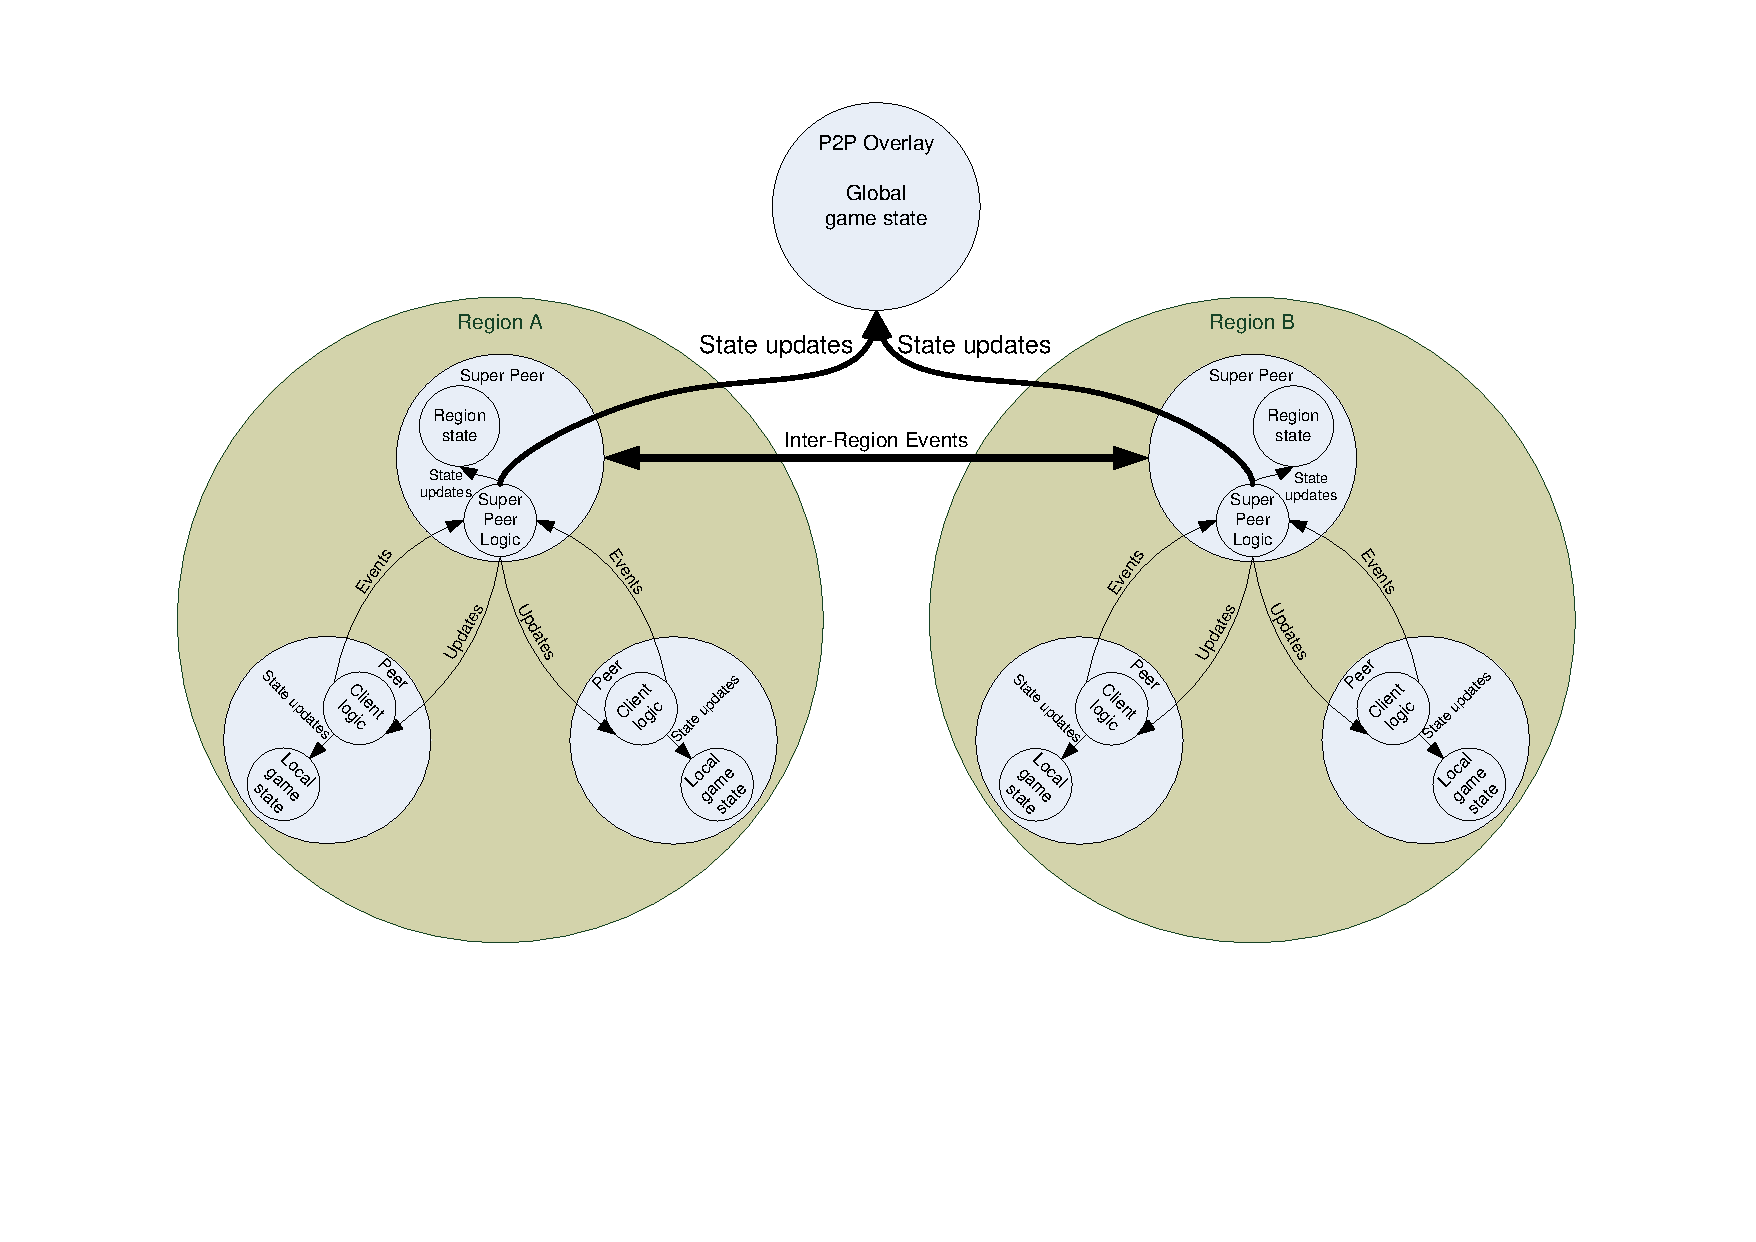
\includegraphics[clip=true, viewport=2cm 5cm 27cm 19.5cm, width=\textwidth]{region_based_CS_CM_P2PO}
 \caption{Hybrid region-based super peer storage with backup overlay storage consistency model}
 \label{fig_cs_region_o_cm}
\end{figure}
%
Figure \ref{fig_cs_region_o_cm} shows a type of Super Peer/Overlay hybrid storage implemented in \cite{zoned_federation}. The model depicted in
Figure \ref{fig_cs_region_o_cm} uses an overlay storage, managed by regional super peers. The world is divided into regions, with each region
controlled by a super peer. The complete region state is cached at every super peer, the same as with super peer storage. There also exists a backup
overlay storage architecture, to which data may be backed up for long term, redundant and secure storage. The hybrid region-based overlay storage
contains many improvements over pure overlay storage as will be discussed in the following sections.

\subsection{Reliability}
\label{hybrid_storage_reliability}

Because of the use of overlay storage for backup, the hybrid region-based storage is almost as reliable as a pure overlay storage. It is classified
as almost as reliable, because there is a delay between when data changes and when it is updated in the overlay. If a super peer fails during this
time and the data was not backed-up to the overlay, that data could be lost. Backup super peers can, however, be implemented as described in Section
\ref{super_peer_storage_reliability} to improve the reliability of the hybrid storage model.

\subsection{Responsiveness}

Because all regional files are cached at super peers, the system is as responsive as super peer storage.

\subsection{Security}

Security in hybrid storage is still an issue, because of the inherent problems of the super peer storage model. Although it is more difficult for
nodes to access and manipulate data stored in the overlay, a malicious node promoted to super peer status may manipulate the region data it controls.

It does seem possible to achieve higher levels of security, by checking data received from super peers, against the data stored in the overlay. Care
should be taken with such a scheme, because the rate of change of data at the super peers might be higher than the rate that data are submitted to
the overlay. Another issue is the time delay between data received from a super peer and data received from the overlay.

\subsection{Fairness}

The issue of unfairness is also still present in hybrid storage. The system is fairer in that all nodes share the load of the overlay storage, but
there still exists the unfairness of the super peer storage. As all data exists in both the overlay storage as well as the super peer storage, the
system is as unfair as super peer storage, because the same quantity of data as in super peer storage is not being distributed evenly amongst all
nodes.

\subsection{Existing architectures}

\begin{figure}[htbp]
 \centering
 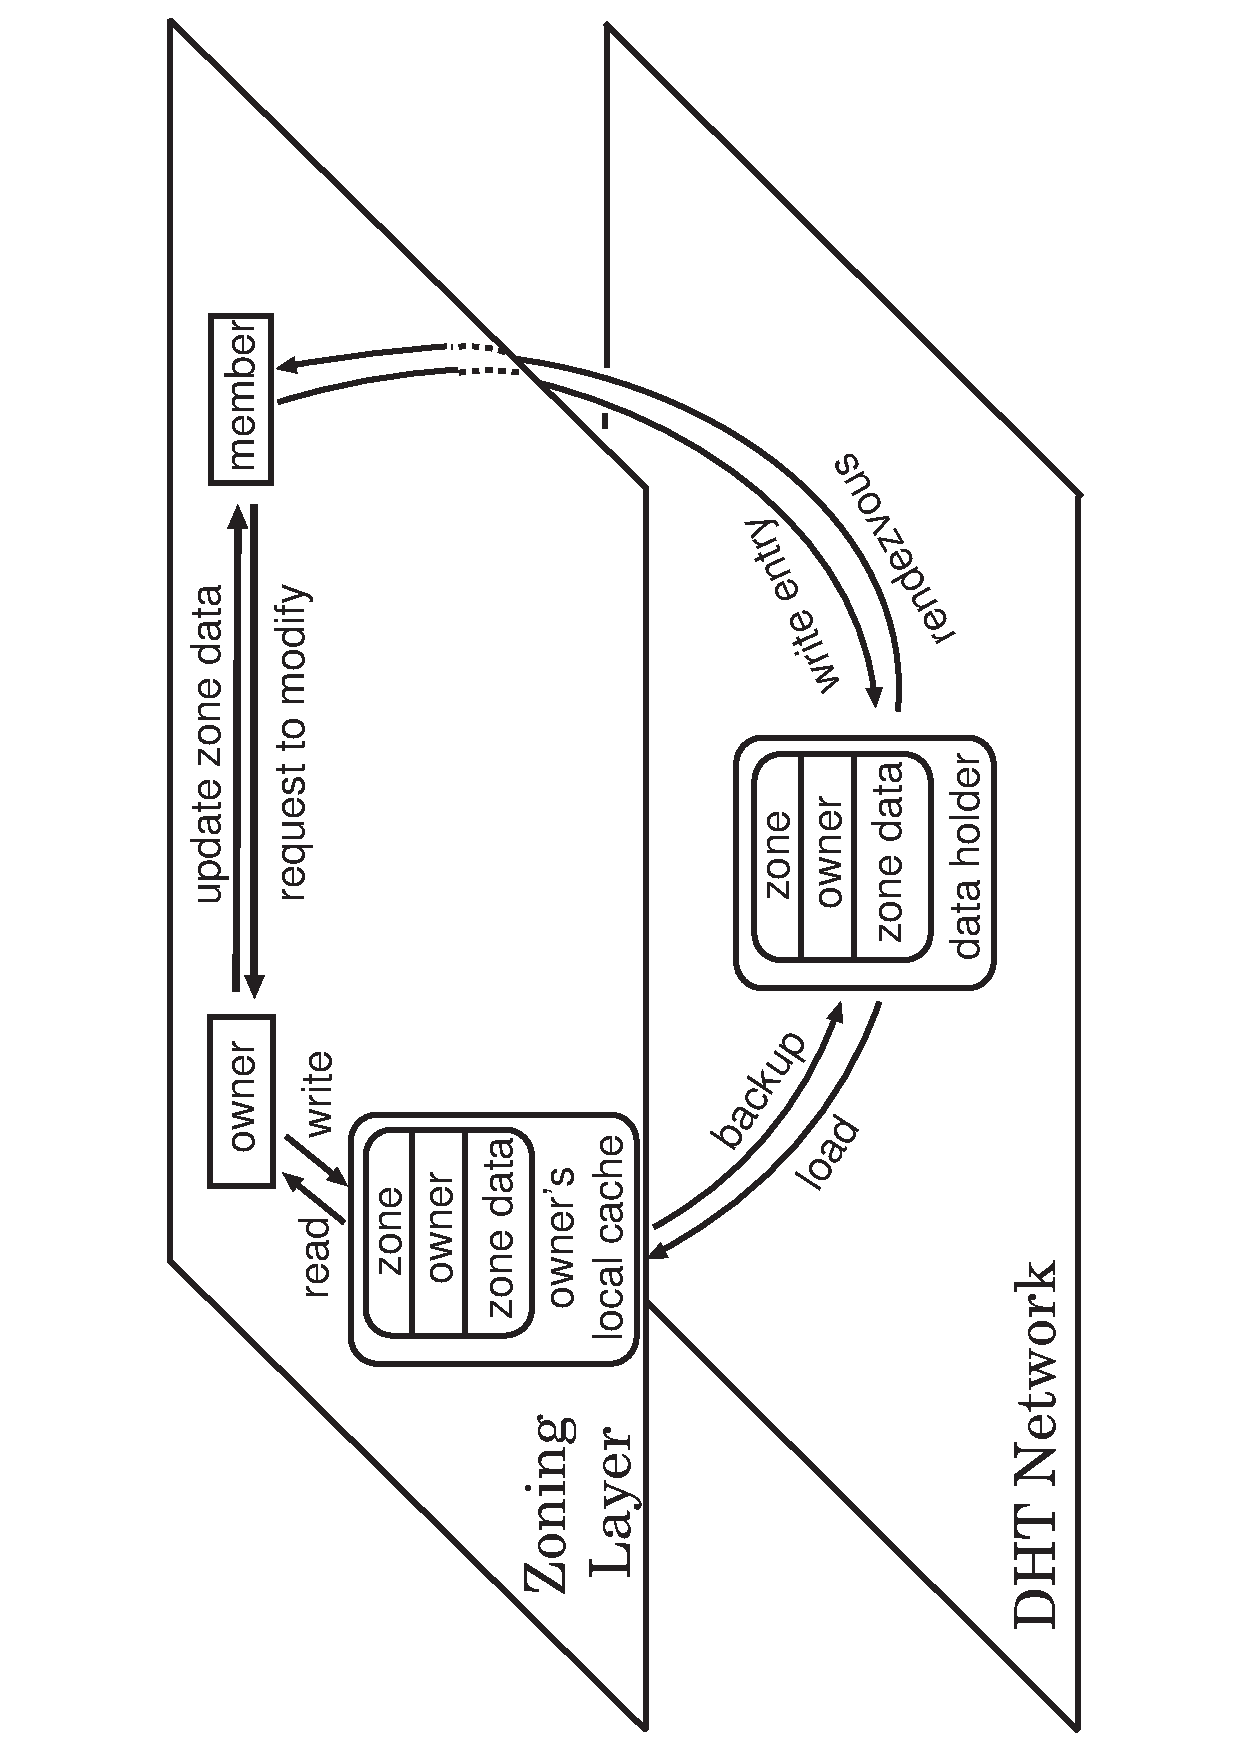
\includegraphics[clip=true, viewport=2cm 0cm 19cm 30cm, angle=-90, width=0.5\columnwidth]{zoned_federation_model}
 \caption{Zoned Federation Model \cite{zoned_federation}}
 \label{fig_zoned_federation_model}
\end{figure}
%
The first hybrid state persistency model for P2P MMVEs was proposed by Iimura et al. in 2004 \cite{zoned_federation} and called the ``Zoned
Federation Model'', shown in Figure \ref{fig_zoned_federation_model}. The regional super peers are called ``Zone Owners'', which handle all events by
clients in their zone or region. In the Zoned Federation model, a Zone Owner acts as the primary storage medium for all object states in the zone or
region. As shown in Figure \ref{fig_cs_region_o_cm}, this is analogous to an update based model, divided into zones. The difference here is that the
game state of all zone owners are regularly backed-up to overlay storage. The zoned federation model can thus be seen as a super peer/overlay storage
hybrid. The super peers storage provides for low latency data storage and the overlay storage provides security and reliability.

An extended abstract, published by GauthierDickey et al. in 2004 \cite{hybrid_storage1}, proposed to distinguish between permanent and ephemeral
data. Permanent data are described as data that should exist at all times and ephemeral data are described as data that need only exist for as long
as its owner is in the game. An item, being dropped by a dispatched NPC, can be considered as ephemeral. When the peer on which the data is hosted
leaves the area, that item can disappear. An example of permanent data is a player's inventory contents, which can further be classified as
participatory data or a player's house, which can be classified as existential data. Participatory data are data that need only be available when a
specific player is in the game and existential data are data that should be available, even when a certain player is not present in the game.

Categorising data by how long and under which circumstances the data should exist, may assist in the design of the storage model. Since ephemeral
data does not have to exist after the player has left the game, it may be stored in primary memory. Participatory data might also be stored on the
player's computer, but security issues will have to be kept in mind. Existential data will have to be stored somewhere other than on the player's
computer, since other players will require the data, even in the absence of the player that might have left the game. GauthierDickey et al. did not
explore how their data classification scheme might be translated into a state persistency model.

\section{Distance-based storage}
\label{distance_based_storage}

%Distance-based - overview
Distance based approaches, such as the Voronoi storage approaches \cite{Buyukkaya_voronoi_state_management}, \cite{Hu_voronoi_IM} and some more
general approaches \cite{colyseus_distance_based}, \cite{solipsis}, store object data on the peer closest to the object in the virtual world. Some
distance metric is used to determine on which node an object should be stored.

\begin{figure}[htbp]
 \centering
 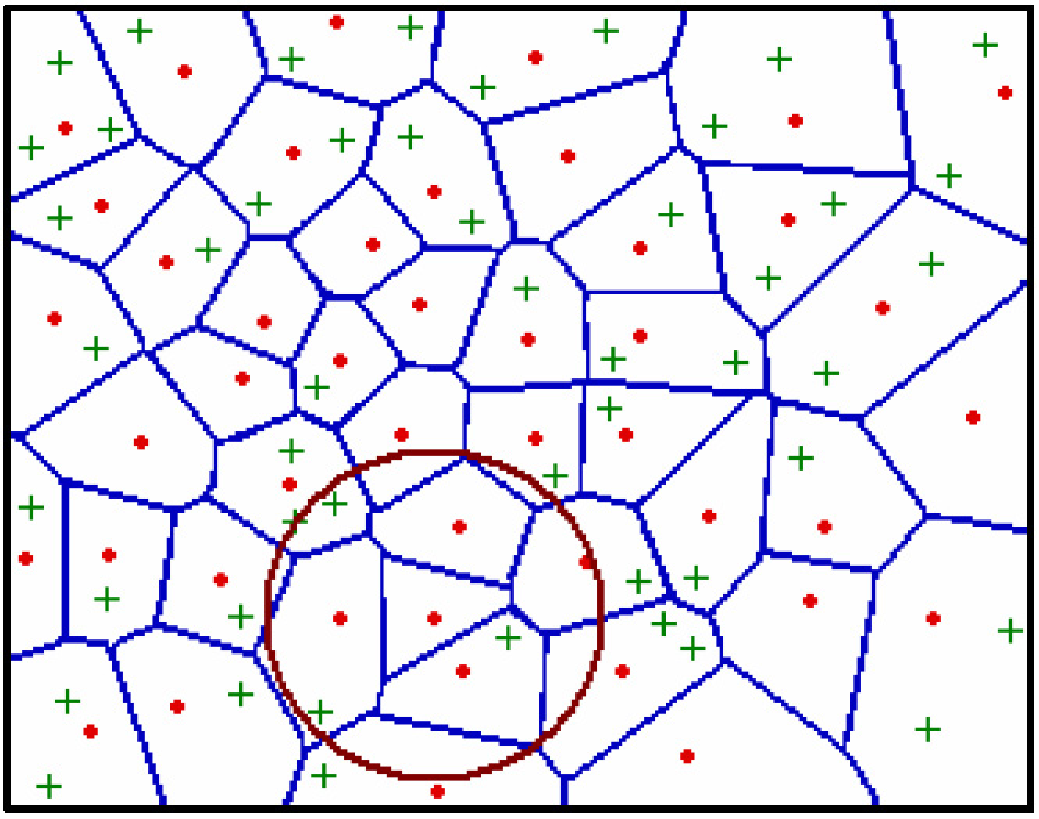
\includegraphics[width=0.4\columnwidth]{voronoi_diagram}
 \caption{Voronoi Diagram \cite{Buyukkaya_voronoi_state_management}}
 \label{fig_voronoi_diagram}
\end{figure}
%
Given a set of points, the Voronoi diagram of the set of points is the partition of the plane, which associates a region around every point in such a
way that all other points contained in the region are closer to the centre point than any other point in the set. Figure \ref{fig_voronoi_diagram}
shows a Voronoi diagram, where the lines define the region boundaries, the dots define the players, which make up the set of points for which the
diagram was calculated, the plus signs represent mutable objects and the circle represents the AoI of a central point in the set.

For the Voronoi approaches, described in more detail in Section \ref{distance_based_existing_archs}, a node controls and hosts all objects within its
Voronoi region. The reasoning is that there is a high probability that the player closest to the object is also the player using the object. Examples
of this are where a player is trading or fighting with an NPC.

\subsection{Responsiveness}

%Distance-based - issues
An issue with the above reasoning is that multiple nodes are usually interacting with a single object. The examples of the NPC monster and trader are
again relevant. Usually many players interact with a trader NPC and usually players attack monster NPCs in groups.

Multiple player interactions are, however, not as big an issue as others have suggested \cite{Fan_deisgn_issues_p2p}. In the best case, the object
being used by a player is also hosted on that player's node. If another player requires use of a remotely hosted object, that player may still
interact with the object, where the host node is now acting as a server to that player. This means that every player hosting an object becomes a
server for that object. In the case where a player interacts with an object hosted locally, there is no object latency. In the case where a player
accesses a remotely hosted object, there is only one hop latency, the same as with a C/S or super peer application.

Issues with this approach stem from the fact the players are constantly moving. When players move, the objects in their regions change. Objects,
therefore, have to be constantly handed over from one peer to another, which might cause significant network traffic. An object in transit might also
delay interaction with that object. Because object transfer introduces overhead into the system, how regularly an object has to be transferred and
whether the number of transferrals produce sufficiently low overhead to implement a real-time game, still have to be investigated.

Voronoi-based storage schemes also become unresponsive when communications are no longer between neighbours, but between two arbitrary nodes in the
Voronoi overlay. When such communications occur, the average required time to route a message is $\OO{N^{1/2}}$ for a two-dimensional configuration.
Advancements have been made that suggest augmenting the Voronoi overlay with additional links to far off nodes to create a small world network. This
reduces the average routing time to $\OO{\log{(N)}}$, the same as for overlay storage \cite{Steiner_voronoi_shortcuts}.

\subsection{Reliability}

Reliability, because of network churn, is still an issue. Nodes will leave the network whenever a player stops playing the game, which makes it a
common occurrence. When nodes leave the network, the objects that are stored on that node should still be accessible to other players. This will
require transferring all objects contained in the leaving node to another object, still present in the network. No papers have yet dealt with the
issue of reliability in a distance-based storage network.

The same solution that is used for overlay storage, namely the presence of redundant peers, might also be implemented for distance storage. Another
structured overlay might be used to implement this redundancy in exactly the same way it is done with hybrid storage mentioned in Section
\ref{hybrid_storage_reliability}.

\subsection{Security}
\label{distance_based_storage_security}

The main issue with the distance based scheme is security. Nodes that have the most interest in an object also have the most interest to manipulate
that object in ways inconsistent with the game rules. When objects are hosted on nodes that have the most interest in them, there will be a strong
drive to try and manipulate these objects. Because these modification are all local, it is also not possible to log the alterations and detect
cheating. Means by which local objects can be secured have to be found or distance based algorithms with quorum need to be investigated.

This security issue is similar to that of super peer storage, in that local data can be accessed, thus circumventing the certification system. With
this circumvention, the objectives of authentication, authorisation, confidentiality, trust, privacy and identity management are all compromised.

\subsection{Fairness}

Distance-based storage is relatively fair as all objects are distributed amongst all nodes. Where the system becomes somewhat unfair is when a node
is nearest to a large number of objects. For Voronoi regioning approaches, this is when a peer's Voronoi region contains many more objects than the
average number of objects hosted by other peers. This might not be a major issue, depending on how long the objects have to be hosted on the
overloaded peer. This will depend on the movement of the overloaded peer as well as that of neighbouring peers. The use of aggregators as a proposed
solution to this problem is discussed in Section \ref{distance_based_existing_archs}.

\subsection{Existing architectures}
\label{distance_based_existing_archs}

%Colyseus, 2006
Bharambe et al. created the Colyseus architecture in 2006 \cite{colyseus_distance_based}. The architecture is designed to support First Person
Shooter (FPS) games and implemented to function with Quake II. Mutable game objects are stored on the peer that is nearest to the object in the game
world. An ``object placer'' component is mentioned, but the details of the placement algorithm are left for future work. The architecture also does
not implement non-volatile state persistency, since this is not required for normal FPS games, where object states need only exist to the end of a
round and where players generally do not leave before the end of the round. This means that object states are only stored in primary memory, until
the end of a game round.

%Solipsis, 2008
The Solipsis architecture was created by Frey et al. in 2008 \cite{solipsis}. The architecture uses Voronoi diagrams to create virtual regions.
Stationary objects are maintained by site nodes until a player picks up an object. When an object is picked up, control of that object is transferred
to the player that picked up the object. The Solipsis architecture focusses on distributed physics computation and when a player gains control of an
object, that player is responsible for the object's physics computations. That player should also save all object state until a new player takes the
object, at which time control is transferred to her. Control can also be transferred back to a site node if an object remains stationary for some
time.

What differentiates the Solipsis distance-based storage from the other architectures presented in this section, is that object states are only
handled by peers as long as those peers directly use an object. At other times, those objects are handled by site nodes. This differs from other
distance-based storage techniques, where all objects that are nearest to a player in the virtual world are controlled by that player.

%Buyukkaya and Abdallah, 2008 and Hu et al., 2008
In 2008, papers were published by Buyukkaya and Abdallah \cite{Buyukkaya_voronoi_state_management}, and Hu et al. \cite{Hu_voronoi_IM}, proposing to
use Voronoi diagrams \cite{voronoi_diagrams_survey} to implement distance-based storage. Voronoi state management schemes host the mutable objects on
the peer in which region the object exists. As peers move around in the virtual world, the Voronoi diagram has to be constantly recalculated and
objects have to be moved to new owner peers as the regions in which they fall change. The significant advantage of the Voronoi approach is that peers
only require connections with their neighbours, and peers within their AoI.

A thesis by Chang also describes the Voronoi approach in more detail and how to achieve game state consistency amongst all nodes in a Voronoi network
\cite{Chang_Voronoi_state_management_masters}. What distinguishes this work from the others is the implementation of a load balancing mechanism. When
peers get overloaded, another, more powerful peer is chosen as an Aggregator. The Aggregator assumes responsibility for a larger area that
encompasses multiple peers. This scheme will reduce the load on peers with minimal resources, but it is uncertain how this would reduce load when
peers with an average number of resources in an area become overloaded.

The works by Buyukkaya and Abdallah, Hu et al., and Chang form part of the VAST project, which is being created to be a fully functional P2P overlay
architecture, using Voronoi diagrams as its basis \cite{VAST}. The reason why state persistency in Voronoi-based P2P MMVEs architectures are mostly
distance-based approaches, is because the Voronoi diagram immediately identifies which objects are closest to a particular peer, and therefore, which
objects that peer has to host. Architectures not making use of Voronoi diagrams still require some other mechanism to identify which objects which
peers should host.

\section{Summary and recommendations}
\label{recommendations}

Supper peer storage can be seen as a C/S type storage implementation, where every region has a super peer that stores all data for that region.
Overlay storage is a fully distributed, P2P approach to storage, where every node stores data as part of a P2P overlay network. Hybrid region based
storage combines super peer and overlay storage to improve the overall storage performance. Distance based storage is a different paradigm that
stores game objects on the nearest node to that game object. This type of storage is usually characterised by the use of Voronoi diagrams to
determine which nodes are nearest to which objects.

Super peer storage is characterised by its high level of responsiveness and ease of implementation. Overlay storage is characterised by its high
level of fairness and reliability. Hybrid region-based storage combines the two previous schemes and has high levels of reliability and
responsiveness. Distance based storage is also very responsive and can be made both reliable and fair.

Security is still an issue for all storage types. Super peer storage has the issues that are usually present in a centralised system, namely low
fairness, security and also not being reliable and not resistant to failure. The main issue with overlay storage is its unresponsiveness, because of
the routing delay in the P2P overlay. Hybrid storage suffers from the disadvantages of super peer storage, namely low fairness and security, due to
all files still stored on super peers. The main issue of distance based storage is security, because players that have the most incentive to alter
object states own those objects.

The different storage types vary greatly in implementation complexity as also shown in Table \ref{tab_storage}. The simplest type of storage to use
is super peer storage, but because of the many issues present, this is not recommended. Only when one is sure that the super peers will not be
overloaded should this storage method be used. There might still be some customers who are unhappy that a few have to serve data to the many.

No recent mention could be found of researchers implementing super peer storage for P2P MMVEs. This could mean that there has been very little
evolution in super peer storage and that super peer storage is currently less mature than other storage schemes. Super peer storage might still be
used for small independent casual games, such as online board games, where a group of friends can implicitly trust each other or where the risk of
cheating is at a minimum. The reason why this storage method is recommended for games from independent developers, is because the scheme is easy to
implement and will not require many resources when used for small games.

For developers who are looking for a simple yet fairly robust storage system to start using in their project, overlay storage is recommended. Overlay
storage can be used for games that do not require low latency data access and would allow for lazy updating of the database. These games will be
lightweight casual and social games. But, depending on the game implementation itself, this storage type might also be used for smaller hardcore
games. Overlay storage will place some restrictions on certain game mechanics, but it is possible that games could be designed around these
restrictions. The primary restriction being that data cannot be immediately retrieved or stored from or to storage.

Examples of overlay storage types that might be used are: PAST, Freenet and Oceanstore and any other overlay storage that is based on a DHT overlay.
Storage based on DHT overlays is still a viable research field and future implementations will improve on the present systems.

Hybrid region-based storage has all the advantages of super peer storage, but with the additional reliability of overlay storage. For this reason, it
is recommended that any game presently requiring high levels of reliability and responsiveness use hybrid storage, instead of super peer or overlay
storage. This storage type currently seems to be the only type applicable to games that require responsive and reliable storage.

%Implementation complexity of hybrid storage
That said, no existing implementations could be found that implement this type of storage for public use. The consequence is that someone who wishes
to use this storage will mostly have to implement it. This can be done by starting out with super peer storage and using a publicly available overlay
storage to augment the super peer storage.

Distance based storage is still fairly immature, but shows a lot of promise. No publicly available implementation could be found for this type of
storage. Where this type of storage was used, it was explained as distance based storage, but most of the details were left out. This storage is,
therefore, not a candidate as a storage technique for developers that are merely looking for a storage system to use presently. This type of storage
does, however, provide a lot of opportunities for research.

\section{Conclusion}
\label{conclusion}

\subsection{Summary}
%Paper summary
After providing an overview of the classic C/S and C/MS state persistency techniques, this survey classified P2P MMVE state persistency techniques
into super peer based, overlay based, distance based and hybrid storage. The advantages and disadvantages of each method were discussed after
identifying key challenges that state persistency techniques have to solve. These challenges are: Reliability, Security, Fairness and Responsiveness.

We conclude that there exists no single state persistency architecture, currently in use, that is suited to P2P MMVEs. None of the storage techniques
reviewed meet the requirements of a real-time distributed application, such as an MMVE. What is required is a state persistency architecture,
specifically geared towards data persistency in P2P MMVEs, that meet all the challenges of the application.

%Reason for paper
This survey was written, because of an identified need for a concise summary of the field of P2P MMVE game state persistency. Many techniques used in
the past were used because of the ease with which they could be integrated into a P2P MMVE. The purpose of this survey is to identify those
techniques and to stimulate further research, using empirical methods to compare the different storage techniques used.

\subsection{Prospective research directions}
%How to address storage challenges
One of three paths may be followed in order to create a storage type that is suitable to modern hardcore MMVEs. The first would be to take a look at
the deficiencies mentioned in the different storage types and to then improve one of these types. The other path is what was seen with hybrid
storage, where multiple types of storage are combined in order to form a new and improved storage type. The third path would be to create a new
storage type, based on some novel insight into the ways in which games are designed.

%What are some of the challenges of the different storage types
What follows is a discussion on what work is required in order to improve the current storage types and attempts to define the gaps present that
should still be solved by future researchers.

For super peer storage to become viable, a means is required to secure the data stored in the super peers and ensure that no super peer is able to
access the data stored. If this issue is solved, the fairness issue still exists, but might be allowable depending on the type of application.

%Overlay storage - reason
Overlay storage is a popular storage method in the literature. This is believed to be more as a consequence of the use of Scribe \cite{scribe} than
any inherit benefit to P2P MMVEs \cite{past_storage_focus}, \cite{Fan_phd}. The reason for using overlay storage in so many implementations seem to
be merely the availability of PAST, after having already decided to use Scribe. In other words, researchers use Scribe for ALM, Scribe runs on
Pastry, and PAST is then a readily available storage implementation which also runs on Pastry.

The applicability of overlay storage to MMVEs is still unknown and further research is required. This paper showed that while PAST is regularly used
in P2P MMVEs, it is not because of the applicability of PAST to P2P MMVEs.

One type of hybrid storage was investigated in this paper, namely overlay/super peer storage, since this is a hybrid type currently seen in P2P
MMVEs. Other hybrid types should also be investigated, for example a distance based/overlay storage hybrid might improve the reliability of distance
based storage. Multi-tiered storage might also be of interest, where players or areas are grouped in some way. One type of storage might then be
implemented amongst the members of a group, with another storage type implemented over all groups. Such a storage type might improve responsiveness
amongst group members, while adding reliability because of an inter-group backup mechanism.

Distance-based storage still seems immature, with many open questions. Currently, distance-based storage is based on Voronoi diagrams, which seem
promising. But Voronoi diagrams only provide for a means to identify which objects should be under a specific node's control. Object migration, which
will occur frequently in this type of storage should still be addressed. The number of migrations should be kept to a minimum to ensure responsive
access to all stored objects.

The storage is also not yet reliable, but it could be possible to add overlay storage as a backup to the system and thereby add reliability. If
voting techniques can be used to update game state, some of the security issues might also be solved. With these two issues addressed, the high
degree of fairness of distance-based storage makes it an excellent candidate to power the P2P MMVEs of the future.

%Performance comparison of storage
An empirical comparison of the performances of the different storage types is also required. It is believed that the metrics presented in this paper
could provide a common basis to use in comparing the different storage types.

%Need for storage characteristics
Research is still required into the characteristics of data stored by MMVEs. This includes how regularly game objects are stored as well as the sizes
of these objects. It is also expected that different read and write patterns exist for different types of game objects. These patterns should be
explored in order to determine what the required performance is for P2P MMVEs storage mechanisms.

It is recommended that C/S MMVE storage patterns initially be investigated to provide a benchmark of the required storage performance for a mature
MMVEs. The storage patterns for a C/S compared to P2P MMVEs might be different. The storage patterns amongst different MMVEs might also differ
greatly, but for an immature field any data is better than no data.

In conclusion, this paper describes a possible new research field with many open questions still to be answered.
